
\section{| 3 Examen des données, prétraitements et extraction des descripteurs}

\subsection{| 3.1 Question}

\begin{lstlisting}
#%% package
import numpy as np
import matplotlib.pyplot as plt

from loadImages import loadImages
from selectFeatureVectors import selectFeatureVectors
from displayFeatures2d import displayFeatures2d
from displayFeatures3d import displayFeatures3d


#%% def preprocessing
def preprocessing():
    # ------------------------------------------------
    # YOUR CODE HERE
    img73, img87 = loadImages()

    plt.figure()
    plt.imshow(img73)
    plt.title("Mer d'Aral (1973)")

    plt.figure()
    plt.imshow(img87)
    plt.title("Mer d'Aral (1987)")

    plt.show()

    featLearn = None
    # ------------------------------------------------
    # ------------------------------------------------
    #%% sortie
    return featLearn,img73,img87
\end{lstlisting}

\begin{figure}[H]
    \centering
    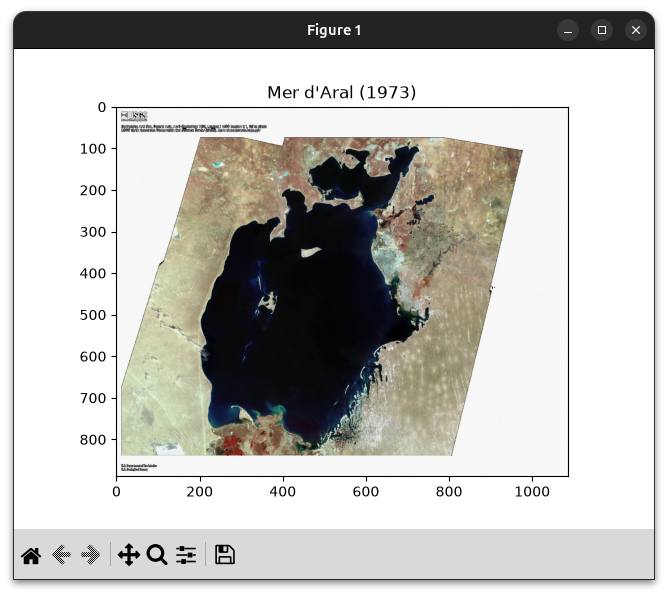
\includegraphics[width=0.75\linewidth]{figure/image.png}
    \label{fig:placeholder}
\end{figure}

\begin{figure}[H]
    \centering
    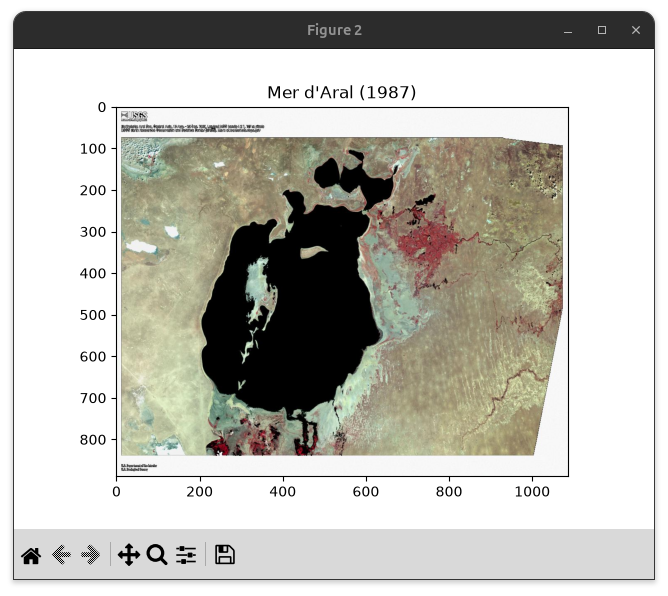
\includegraphics[width=0.75\linewidth]{figure/image1.png}
    \label{fig:placeholder}
\end{figure}


\subsection{| 3.2 Question}

R: On observe une diminution de la surface de la mer d’Aral entre 1973 et 1987. Les images sont codées en RGB. Chaque pixel possède trois composantes (rouge, vert et bleu), avec des valeurs comprises entre 0 et 255.


\subsection{| 3.3 Question}
R: L’espace des descripteurs est de dimension 3, parce que chaque pixel est représenté par trois composantes: rouge, vert et bleu.

\subsection{| 3.4 Question}

\begin{lstlisting}
#%% package
import numpy as np
import matplotlib.pyplot as plt

from loadImages import loadImages
from selectFeatureVectors import selectFeatureVectors
from displayFeatures2d import displayFeatures2d
from displayFeatures3d import displayFeatures3d


#%% def preprocessing
def preprocessing():
    # ------------------------------------------------
    # YOUR CODE HERE
    img73, img87 = loadImages()

    img73 = img73[75:840, :, :]
    img87 = img87[75:840, :, :]

    plt.figure()
    plt.imshow(img73)
    plt.title("Mer d'Aral (1973)")

    plt.figure()
    plt.imshow(img87)
    plt.title("Mer d'Aral (1987)")

    plt.show()

    print("Dimensions 1973:", img73.shape)
    print("Dimensions 1987:", img87.shape)

    featLearn = None
    # ------------------------------------------------
    # ------------------------------------------------
    #%% sortie
    return featLearn,img73,img87
\end{lstlisting}

\begin{figure}[H]
    \centering
    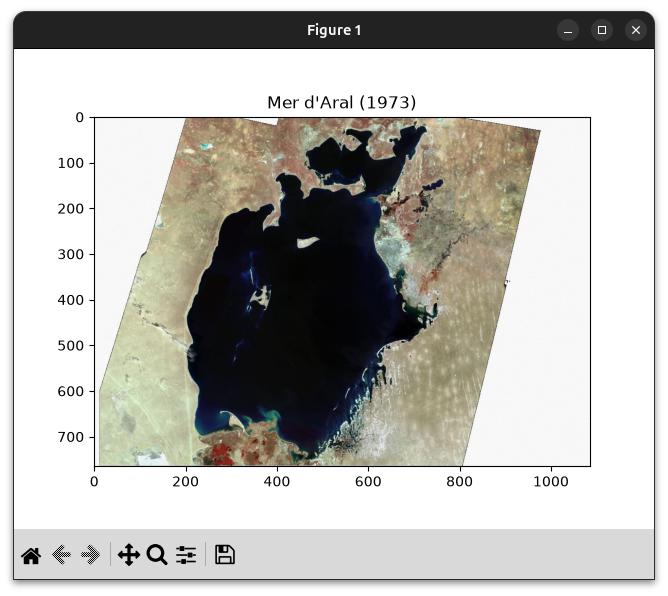
\includegraphics[width=0.75\linewidth]{figure/image3.png}
    \label{fig:placeholder}
\end{figure}

\begin{figure}[H]
    \centering
    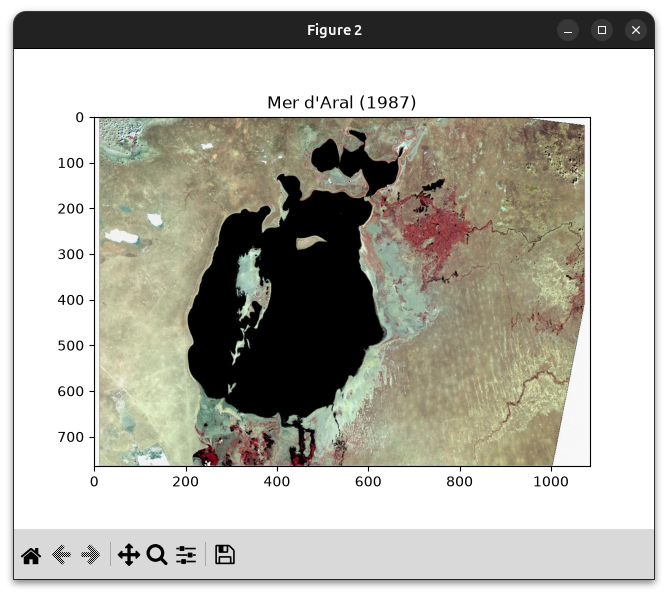
\includegraphics[width=0.75\linewidth]{figure/image4.png}
    \label{fig:placeholder}
\end{figure}

\begin{figure}[H]
    \centering
    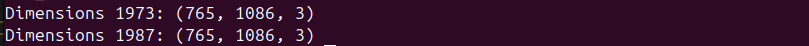
\includegraphics[width=0.75\linewidth]{figure/image5.png}
    \label{fig:placeholder}
\end{figure}



\section{| 4 Constitution d’un ensemble de données d’apprentissage}


\subsection{| 4.1 Question}

\begin{lstlisting}
#%% package
import numpy as np
import matplotlib.pyplot as plt

from loadImages import loadImages
from selectFeatureVectors import selectFeatureVectors
from displayFeatures2d import displayFeatures2d
from displayFeatures3d import displayFeatures3d


#%% def preprocessing
def preprocessing():
    # ------------------------------------------------
    # YOUR CODE HERE
    # Question 3.1
    img73, img87 = loadImages()

    # Question 3.4
    img73 = img73[75:840, :, :]
    img87 = img87[75:840, :, :]

    # Question 4.1
    featLearn, nbPix, nbFeat = selectFeatureVectors(img73, 500)

    plt.figure()
    plt.imshow(img73)
    plt.title("Mer d'Aral (1973)")

    plt.figure()
    plt.imshow(img87)
    plt.title("Mer d'Aral (1987)")

    plt.show()

    print("Dimensions 1973:", img73.shape)
    print("Dimensions 1987:", img87.shape)

    print("\nNombre de donnees d'apprentissage:", nbPix)
    print("Nombre de descripteurs:", nbFeat)
    print("Dimensions de featLearn:", featLearn.shape)
    # ------------------------------------------------
    # ------------------------------------------------
    #%% sortie
    return featLearn,img73,img87
\end{lstlisting}

R: On obtient 1662 données d’apprentissage.

\begin{figure}[H]
    \centering
    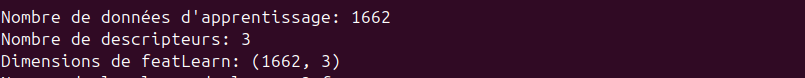
\includegraphics[width=0.75\linewidth]{figure/image6.png}
    \label{fig:placeholder}
\end{figure}


\section{| 5 Première analyse des données}


\subsection{| 5.1 Question}

\begin{lstlisting}
#%% package
import numpy as np
import matplotlib.pyplot as plt

from loadImages import loadImages
from selectFeatureVectors import selectFeatureVectors
from displayFeatures2d import displayFeatures2d
from displayFeatures3d import displayFeatures3d


#%% def preprocessing
def preprocessing():
    # ------------------------------------------------
    # YOUR CODE HERE
    # Question 3.1
    img73, img87 = loadImages()

    # Question 3.4
    img73 = img73[75:840, :, :]
    img87 = img87[75:840, :, :]

    # Question 4.1
    featLearn, nbPix, nbFeat = selectFeatureVectors(img73, 500)

    # Question 5.1
    displayFeatures2d(featLearn)
    displayFeatures3d(featLearn)

    plt.show()

    plt.figure()
    plt.imshow(img73)
    plt.title("Mer d'Aral (1973)")

    plt.figure()
    plt.imshow(img87)
    plt.title("Mer d'Aral (1987)")

    plt.show()

    print("Dimensions 1973:", img73.shape)
    print("Dimensions 1987:", img87.shape)

    print("\nNombre de donnees d'apprentissage:", nbPix)
    print("Nombre de descripteurs:", nbFeat)
    print("Dimensions de featLearn:", featLearn.shape)
    # ------------------------------------------------
    # ------------------------------------------------
    #%% sortie
    return featLearn,img73,img87
\end{lstlisting}

\begin{figure}[H]
    \centering
    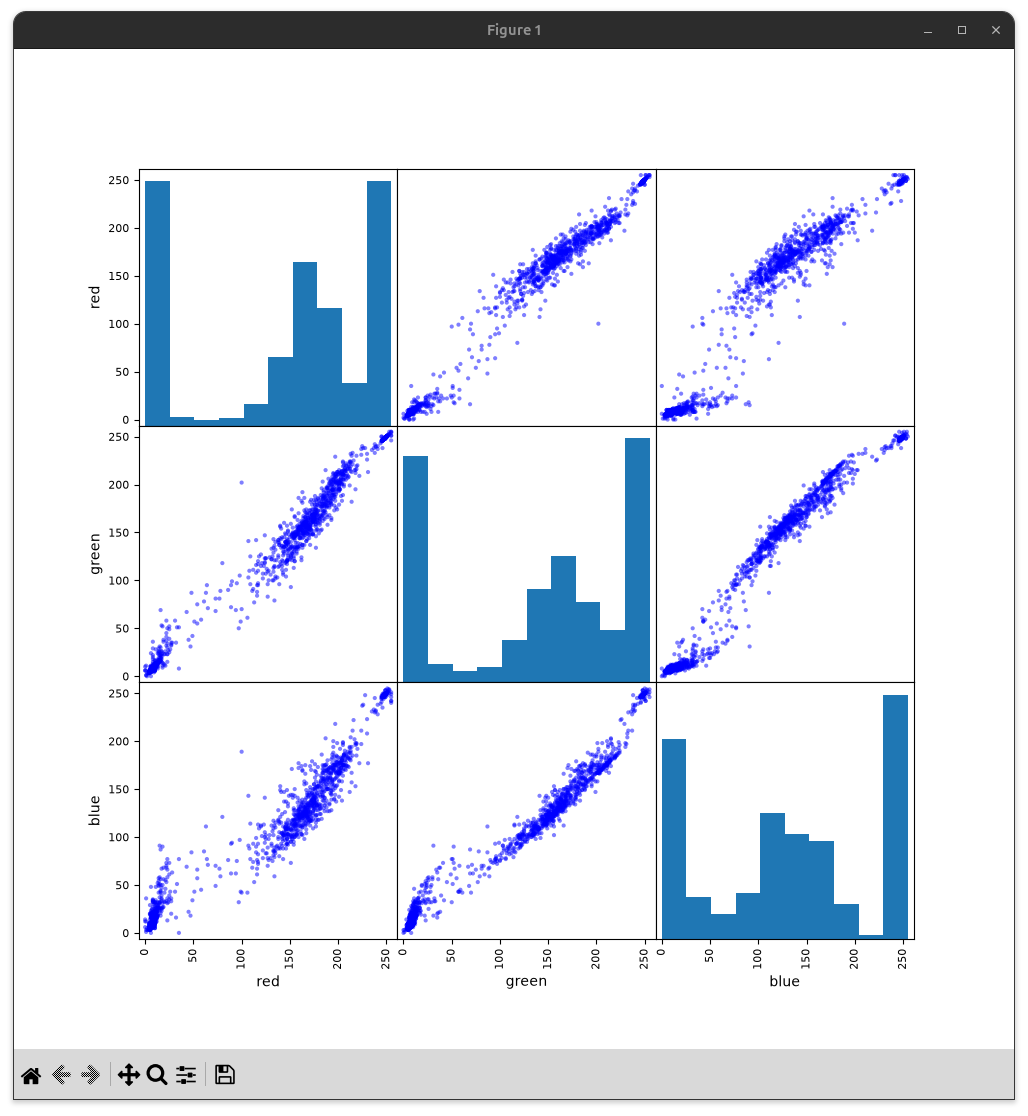
\includegraphics[width=0.75\linewidth]{figure/image7.png}
    \label{fig:placeholder}
\end{figure}

\begin{figure}[H]
    \centering
    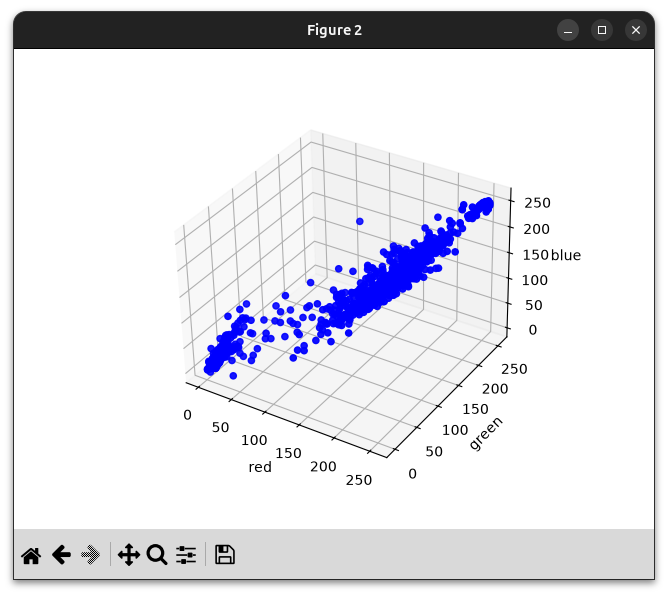
\includegraphics[width=0.75\linewidth]{figure/image8.png}
    \label{fig:placeholder}
\end{figure}


\subsection{| 5.2 Question}

R: Les histogrammes montrent la distribution des valeurs des trois composantes RGB. On observe concentrations de valeurs, proches de 0, entre 100 et 200, et proches de 255. On distingue quelques groupes de pixels selon leurs couleurs : les valeurs faibles correspondent principalement à l’eau, les valeurs intermédiaires au sol et à la végétation, et les valeurs élevées aux zones très claires et au fond blanc de l’image.

\section{| 6 Approche non supervisée par la méthode des k-means}

\subsection{| 6.1 Question}

R: La méthode des centres mobiles consiste à regrouper les données en K classes selon leurs ressemblances.

On initialise K centres, puis chaque point est associé au centre le plus proche. Ensuite, on recalcule les centres avec la moyenne des points de chaque groupe. On répète ces étapes jusqu'à ce que les centres se stabilisent.

\subsection{| 6.2 Question}

unsupervisedTraining.py:
\begin{lstlisting}
#%% package
import numpy as np
from sklearn.cluster import KMeans
from sklearn.mixture import GaussianMixture

#%% def unsupervisedTraining
def unsupervisedTraining(featLearn, method='kmeans'):
    ''' apprentissage avec la fonction KMeans() et GaussianMixture 
    de scikit-learn :
    - featLearn est la matrice de l'ensemble d'apprentissage
    - method: type d'algorithme de Machine Learning utilise (KMeans et GaussianMixture) 
    - nbCluster est le nombre de cluster = nombre de classes rentre par l'utilisateur en debut de fonction
    
    - renvoie model: le modele de classement ou classifieur
    '''
    
    # fixer le nombre de classes
    answer = input('nombre de classes:')
    nbCluster = int(answer)
    
    if method == 'kmeans':

    # ------------------------------------------------
    # YOUR CODE HERE
        model = KMeans(
            n_clusters=nbCluster,
            init='k-means++',
            n_init=10,
            max_iter=300,
            random_state=42)
        
        model.fit(featLearn)
    # ------------------------------------------------
    # ------------------------------------------------

    elif method == 'gmm':
    
    # ------------------------------------------------
    # YOUR CODE HERE
        raise NotImplementedError("GMM pas encore implemente")
    
    # ------------------------------------------------
    # ------------------------------------------------
    # sortie
    return model
\end{lstlisting}

aralsea\_main.py
\begin{lstlisting}
#%% Machine Learning Class - Exercise Aral Sea Surface Estimation

# package
import numpy as np
import matplotlib.pyplot as plt

plt.ioff() # to see figure avant input

# ------------------------------------------------
# YOUR CODE HERE
from preprocessing import preprocessing
from unsupervisedTraining import unsupervisedTraining
# ------------------------------------------------
# ------------------------------------------------
#%% Examen des donnees, pretraitements et extraction des descripteurs
# Chargement des donnees et pretraitements
featLearn,img73,img87 = preprocessing()

#%% Apprentissage / Learning / Training
# Apprentissage de la fonction de classement

# ------------------------------------------------
# YOUR CODE HERE
# Question 6.2
model = unsupervisedTraining(featLearn, method='kmeans')

print("Centres des clusters:", model.cluster_centers_)
print("Nombre d'iterations:", model.n_iter_)
print("Inertie:", model.inertia_)
\end{lstlisting}

\begin{figure}[H]
    \centering
    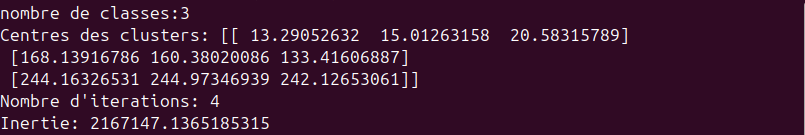
\includegraphics[width=0.75\linewidth]{figure/image9.png}
    \label{fig:placeholder}
\end{figure}

R: On utilise la fonction `KMeans()` de scikit-learn pour créer un modèle de classification non supervisée. Ensuite, on utilise `fit()` pour entraîner le modèle avec les données RGB.
Les principaux paramètres sont `n\_clusters`, qui définit le nombre de classes, `init`, qui définit l'initialisation des centres, `n\_init`, qui définit le nombre d'initialisations, et `max\_iter`, qui limite le nombre d'itérations. Le paramètre `random\_state` permet de reproduire les résultats.

\subsection{| 6.3 Question}

\begin{lstlisting}
# prediction des labels sur la base d'apprentissage

# ------------------------------------------------
# YOUR CODE HERE
# Question 6.3
labelLearn = model.predict(featLearn)

print("Dimensions des labels:", labelLearn.shape)
print("Classes identifiees:", np.unique(labelLearn))
\end{lstlisting}

\begin{figure}[H]
    \centering
    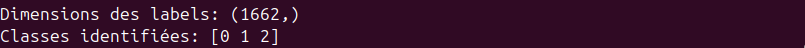
\includegraphics[width=0.75\linewidth]{figure/image10.png}
    \label{fig:placeholder}
\end{figure}

\subsection{| 6.4 Question}

\begin{lstlisting}
# Visualisation des resultats

# ------------------------------------------------
# YOUR CODE HERE
# Question 6.4
displayFeatures2d(featLearn, labelLearn)
displayFeatures3d(featLearn, labelLearn)

plt.show()
\end{lstlisting}

k = 3.
\begin{figure}[H]
    \centering
    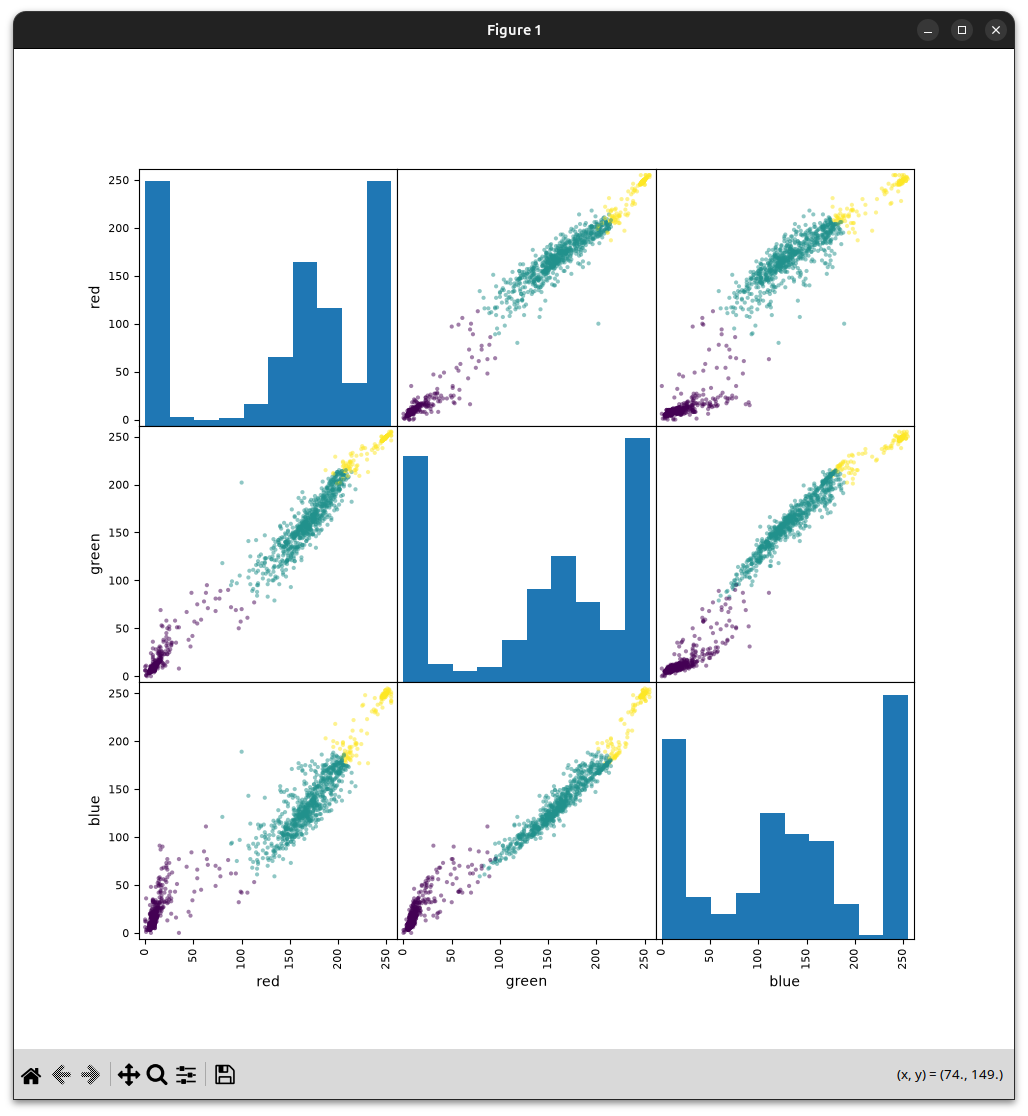
\includegraphics[width=0.75\linewidth]{figure/image11.png}
    \label{fig:placeholder}
\end{figure}
\begin{figure}[H]
    \centering
    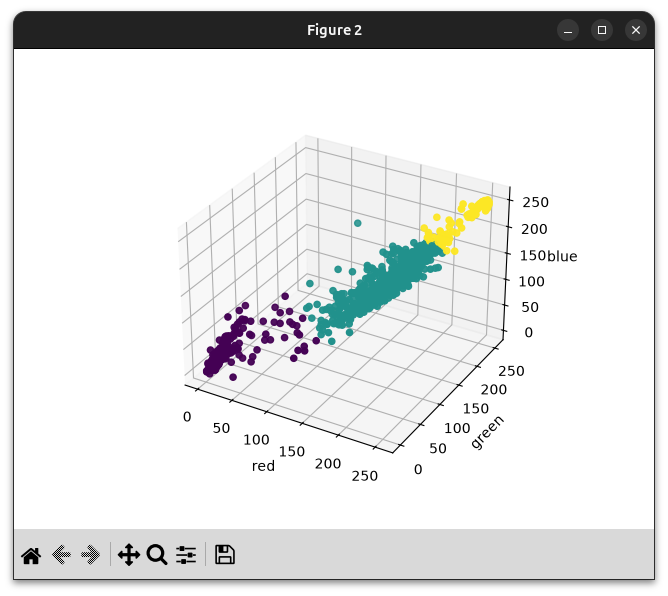
\includegraphics[width=0.75\linewidth]{figure/image12.png}
    \label{fig:placeholder}
\end{figure}

k = 4.
\begin{figure}[H]
    \centering
    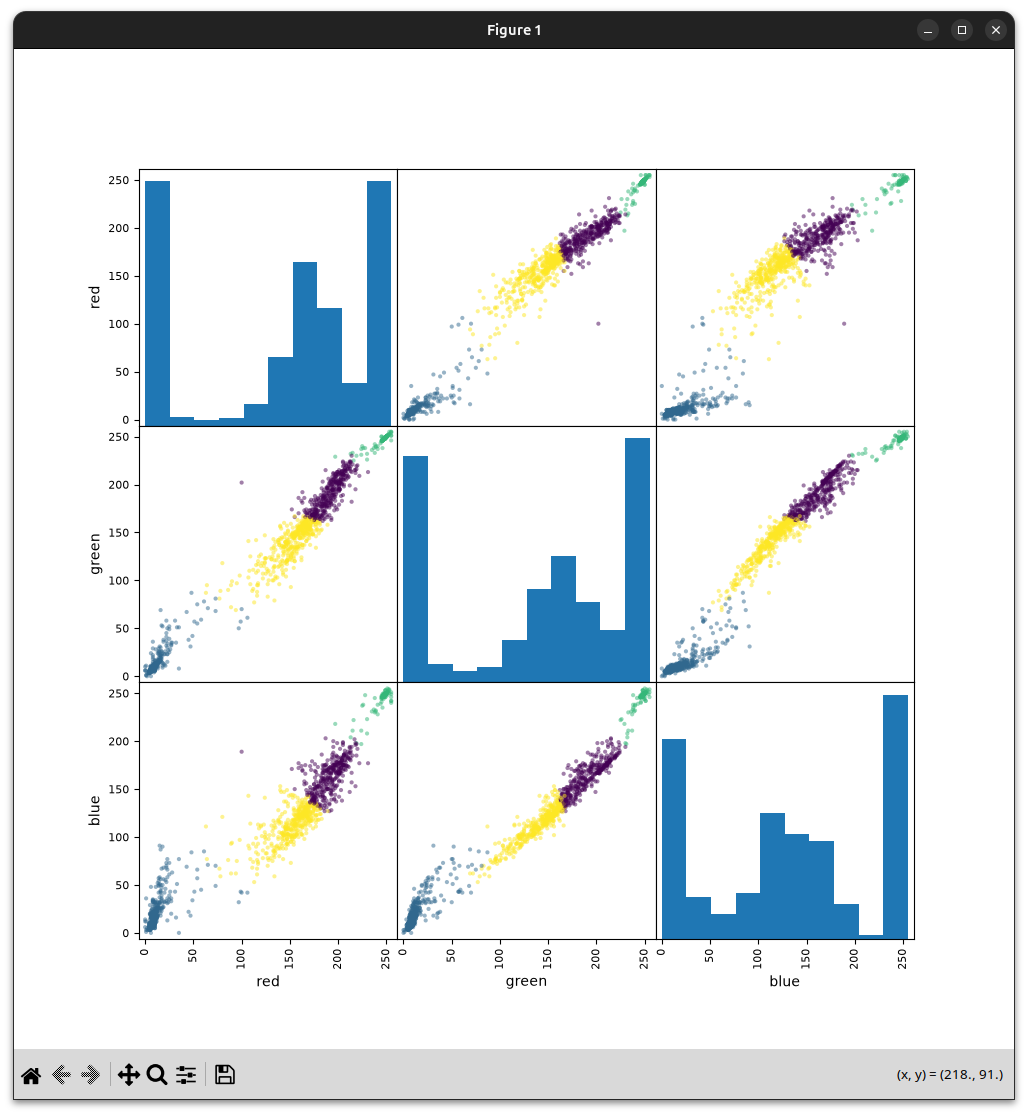
\includegraphics[width=0.75\linewidth]{figure/image13.png}
    \label{fig:placeholder}
\end{figure}
\begin{figure}[H]
    \centering
    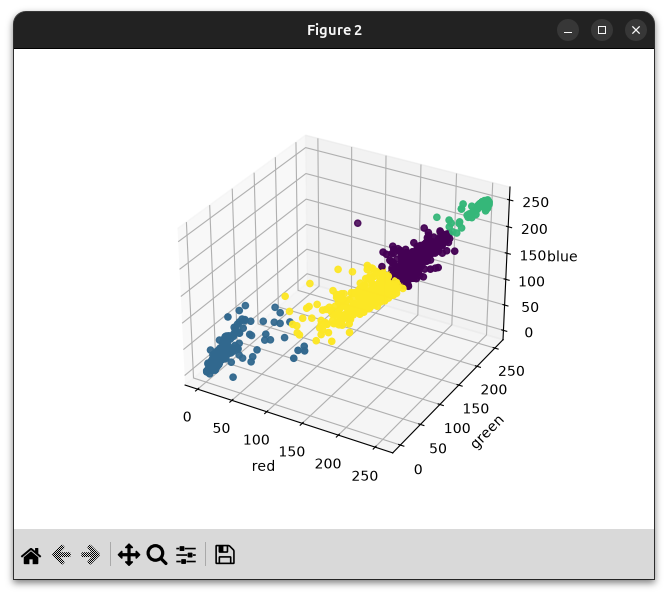
\includegraphics[width=0.75\linewidth]{figure/image14.png}
    \label{fig:placeholder}
\end{figure}

k = 5.
\begin{figure}[H]
    \centering
    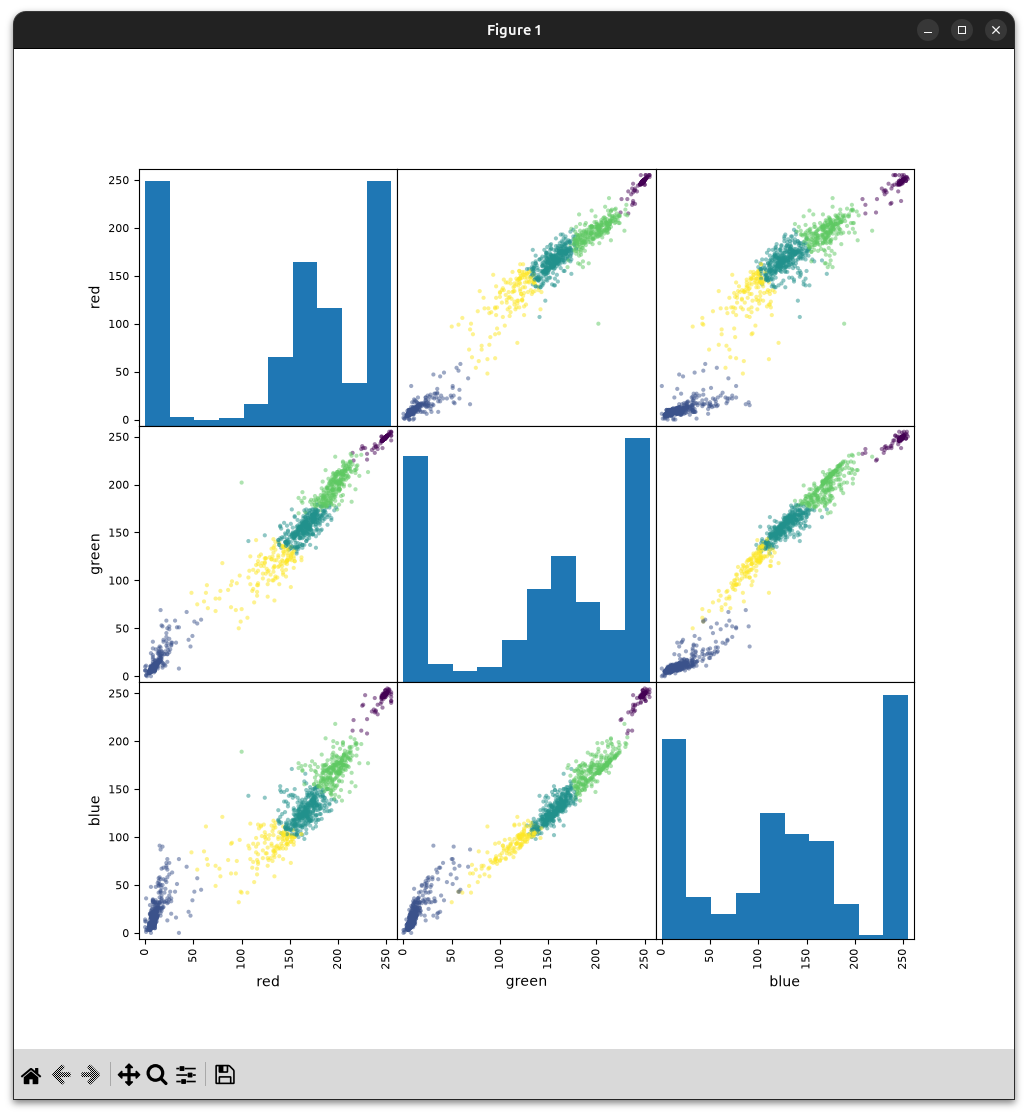
\includegraphics[width=0.75\linewidth]{figure/image15.png}
    \label{fig:placeholder}
\end{figure}
\begin{figure}[H]
    \centering
    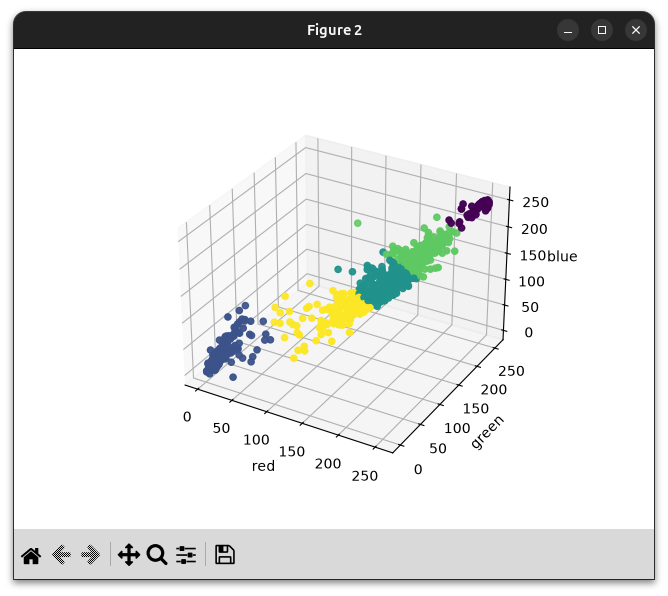
\includegraphics[width=0.75\linewidth]{figure/image16.png}
    \label{fig:placeholder}
\end{figure}

R: On a testé K-means avec 3, 4 et 5 classes. Avec K = 3, on observe trois groupes principaux correspondant aux pixels sombres, intermédiaires et clairs.
Quand on augmente le nombre de classes, les groupes sont divisés en plusieurs sous-groupes. Pour notre objectif, K = 3 semble suffisant pour distinguer les pixels de l'eau des autres régions.

\subsection{| 6.5 Question}

aralsea\_main.py:
\begin{lstlisting}
#%% Classement et estimation de la diminution de surface
# Classifying / Predicting / Testing

# mise en forme de l'image de 1973 et 1987 en matrice Num Pixels / Val Pixels

# ------------------------------------------------
# YOUR CODE HERE
# Question 6.5
nbPix73 = img73.shape[0] * img73.shape[1]
nbPix87 = img87.shape[0] * img87.shape[1]

feat73 = img73.reshape((nbPix73, 3))
feat87 = img87.reshape((nbPix87, 3))

print("Dimensions des descripteurs 1973:", feat73.shape)
print("Dimensions des descripteurs 1987:", feat87.shape)

label73 = unsupervisedClassifying(model, feat73)
label87 = unsupervisedClassifying(model, feat87)

print("Dimensions des labels 1973:", label73.shape)
print("Dimensions des labels 1987:", label87.shape)

print("Classes 1973:", np.unique(label73))
print("Classes 1987:", np.unique(label87))
\end{lstlisting}

unsupervisedClassifying.py:
\begin{lstlisting}
#%% package
import numpy as np
from sklearn.cluster import KMeans


#%% def unsupervisedClassifying
def unsupervisedClassifying(model, feat):
    ''' classement/prediction a partir d'un modele de classement non supervise
    feat est la matrice du jeu de donnees a classer
    label est la classe predite
    '''
	
	# ------------------------------------------------
	# YOUR CODE HERE
    label = model.predict(feat)
	# ------------------------------------------------
	# sortie
    return label
\end{lstlisting}

\begin{figure}[H]
    \centering
    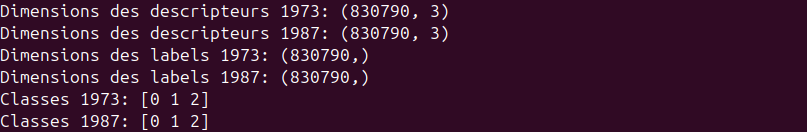
\includegraphics[width=0.75\linewidth]{figure/image17.png}
    \label{fig:placeholder}
\end{figure}

\subsection{| 6.6 Question}

\begin{lstlisting}
# Classement des deux jeux de donnees et visualisation des resultats en image

# ------------------------------------------------
# YOUR CODE HERE
# Question 6.6
plt.figure()
imgLabel73, imgplot73 = displayImageLabel(label73, img73)
plt.title("Classification K-means - 1973")

plt.figure()
imgLabel87, imgplot87 = displayImageLabel(label87, img87)
plt.title("Classification K-means - 1987")

plt.show()
\end{lstlisting}

\begin{figure}[H]
    \centering
    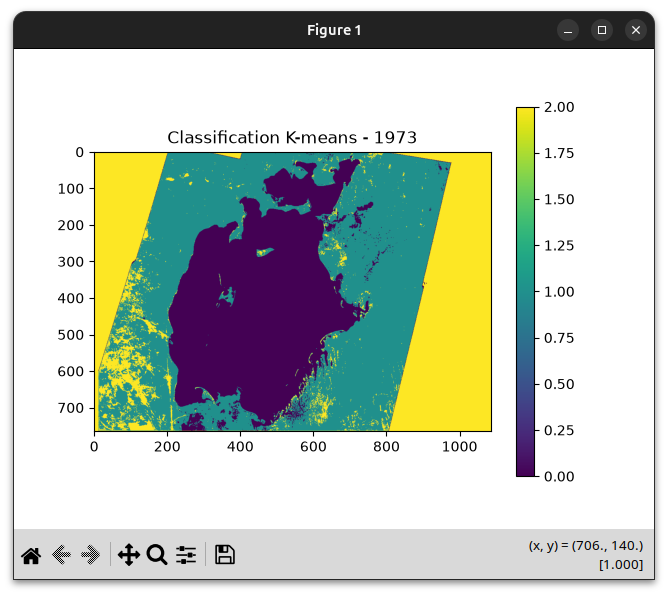
\includegraphics[width=0.75\linewidth]{figure/image18.png}
    \label{fig:placeholder}
\end{figure}

\begin{figure}[H]
    \centering
    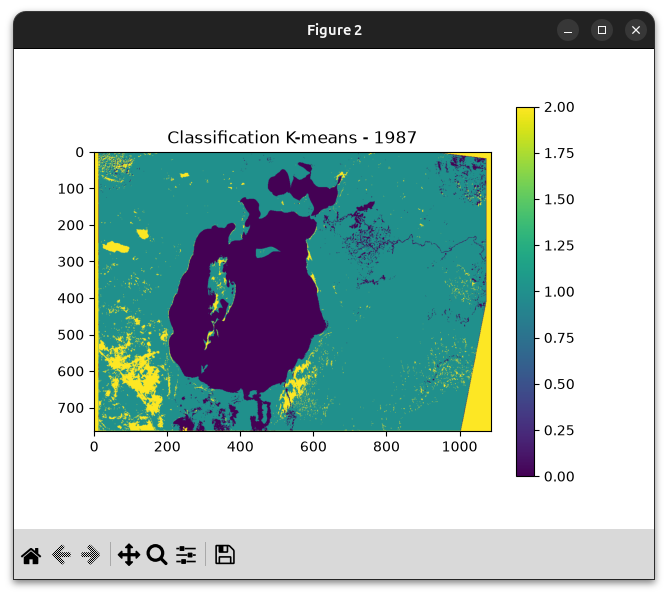
\includegraphics[width=0.75\linewidth]{figure/image19.png}
    \label{fig:placeholder}
\end{figure}

\subsection{| 6.7 Question}

\begin{lstlisting}
#%% Estimation de la surface perdue
answer = input('Numero de la classe de la mer ? ')
cl_mer = int(answer)

# ------------------------------------------------
# YOUR CODE HERE
# Question 6.7
surface73 = np.sum(label73 == cl_mer)
surface87 = np.sum(label87 == cl_mer)

diminution = (surface73 - surface87) / surface73 * 100

print("\n--- Estimation de la surface de la mer d'Aral ---")
print("Nombre de pixels en 1973:", surface73)
print("Nombre de pixels en 1987:", surface87)
print(f"Diminution de la surface: {diminution:.2f} %")
\end{lstlisting}

\begin{figure}[H]
    \centering
    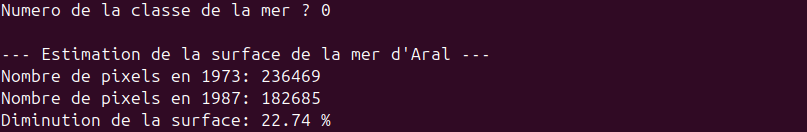
\includegraphics[width=0.75\linewidth]{figure/image20.png}
    \label{fig:placeholder}
\end{figure}

R: On a identifié que la classe 0 correspond principalement à l'eau de la mer d'Aral.

On a ensuite compté le nombre de pixels appartenant à cette classe dans les images de 1973 et 1987.

On obtient une diminution d'environ  22,74 \% entre 1973 et 1987.

\subsection{| 6.8 Question}

k = 3.
\begin{figure}[H]
    \centering
    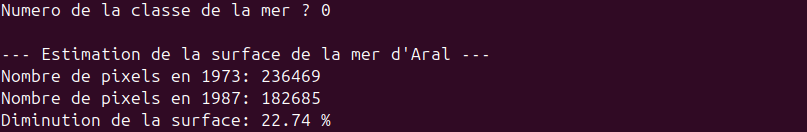
\includegraphics[width=0.75\linewidth]{figure/image20.png}
    \label{fig:placeholder}
\end{figure}

k = 4.
\begin{figure}[H]
    \centering
    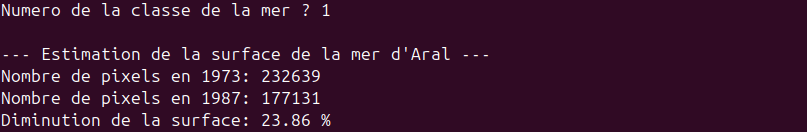
\includegraphics[width=0.75\linewidth]{figure/image21.png}
    \label{fig:placeholder}
\end{figure}

k = 5.
\begin{figure}[H]
    \centering
    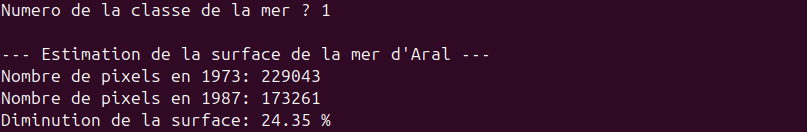
\includegraphics[width=0.75\linewidth]{figure/image22.png}
    \label{fig:placeholder}
\end{figure}

R: On obtient une diminution de la surface de la mer d'Aral de 22,74 \% pour K = 3, 23,86 \% pour K = 4 et 24,35 \% pour K = 5.

On remarque que le pourcentage estimé augmente légèrement avec le nombre de classes. 

\section{| 7 Approche non-supervisée par GMM}


\subsection{| 7.1 Question}

R: Le GMM est une méthode d'apprentissage non supervisé qui regroupe les données à partir de plusieurs distributions gaussiennes.

Chaque gaussienne est représentée par une moyenne, une matrice de covariance et un poids. Contrairement au K-means, le GMM calcule la probabilité qu'un point appartienne à chaque classe.

L'apprentissage utilise l'algorithme EM (Expectation-Maximization), qui fonctionne en deux étapes :

E-step : calculer les probabilités d'appartenance de chaque point aux différentes gaussiennes.

M-step : mettre à jour les moyennes, les covariances et les poids à partir de ces probabilités.

Ces deux étapes sont répétées jusqu'à la convergence du modèle. Ensuite, chaque pixel est classé dans le groupe ayant la probabilité la plus élevée.

\subsection{| 7.2 Question}

unsupervisedTraining.py:
\begin{lstlisting}
#%% package
import numpy as np
from sklearn.cluster import KMeans
from sklearn.mixture import GaussianMixture

#%% def unsupervisedTraining
def unsupervisedTraining(featLearn, method='kmeans'):
    ''' apprentissage avec la fonction KMeans() et GaussianMixture 
    de scikit-learn :
    - featLearn est la matrice de l'ensemble d'apprentissage
    - method: type d'algorithme de Machine Learning utilise (KMeans et GaussianMixture) 
    - nbCluster est le nombre de cluster = nombre de classes rentre par l'utilisateur en debut de fonction
    
    - renvoie model: le modele de classement ou classifieur
    '''
    
    # fixer le nombre de classes
    answer = input('nombre de classes:')
    nbCluster = int(answer)
    
    if method == 'kmeans':

    # ------------------------------------------------
    # YOUR CODE HERE
        model = KMeans(
            n_clusters=nbCluster,
            init='k-means++',
            n_init=10,
            max_iter=300,
            random_state=42)
        
        model.fit(featLearn)
    # ------------------------------------------------
    # ------------------------------------------------

    elif method == 'gmm':
    
    # ------------------------------------------------
    # YOUR CODE HERE
        # Question 7.2
        model = GaussianMixture(
            n_components=nbCluster,
            covariance_type='full',
            n_init=10,
            max_iter=300,
            random_state=42)

        model.fit(featLearn)
    
    # ------------------------------------------------
    # ------------------------------------------------
    # sortie
    return model
\end{lstlisting}

aralsea\_main.py:
\begin{lstlisting}
#%% Apprentissage / Learning / Training
# Apprentissage de la fonction de classement

# ------------------------------------------------
# YOUR CODE HERE
# Question 6.2 / 7.2
# model = unsupervisedTraining(featLearn, method='kmeans')
model = unsupervisedTraining(featLearn, method='gmm')

# print("Centres des clusters:", model.cluster_centers_)
# print("Nombre d'iterations:", model.n_iter_)
# print("Inertie:", model.inertia_)
print("Moyennes des gaussiennes:")
print(model.means_)

print("Poids des gaussiennes:")
print(model.weights_)

print("Nombre d'iterations:", model.n_iter_)
print("Convergence:", model.converged_)
\end{lstlisting}

INFORMATION IMPORTANTE: J'ai oublié de changer le titres des figures pour le question 7.4, donc elles sont encore intitulées "Classification K-means".

\begin{figure}[H]
    \centering
    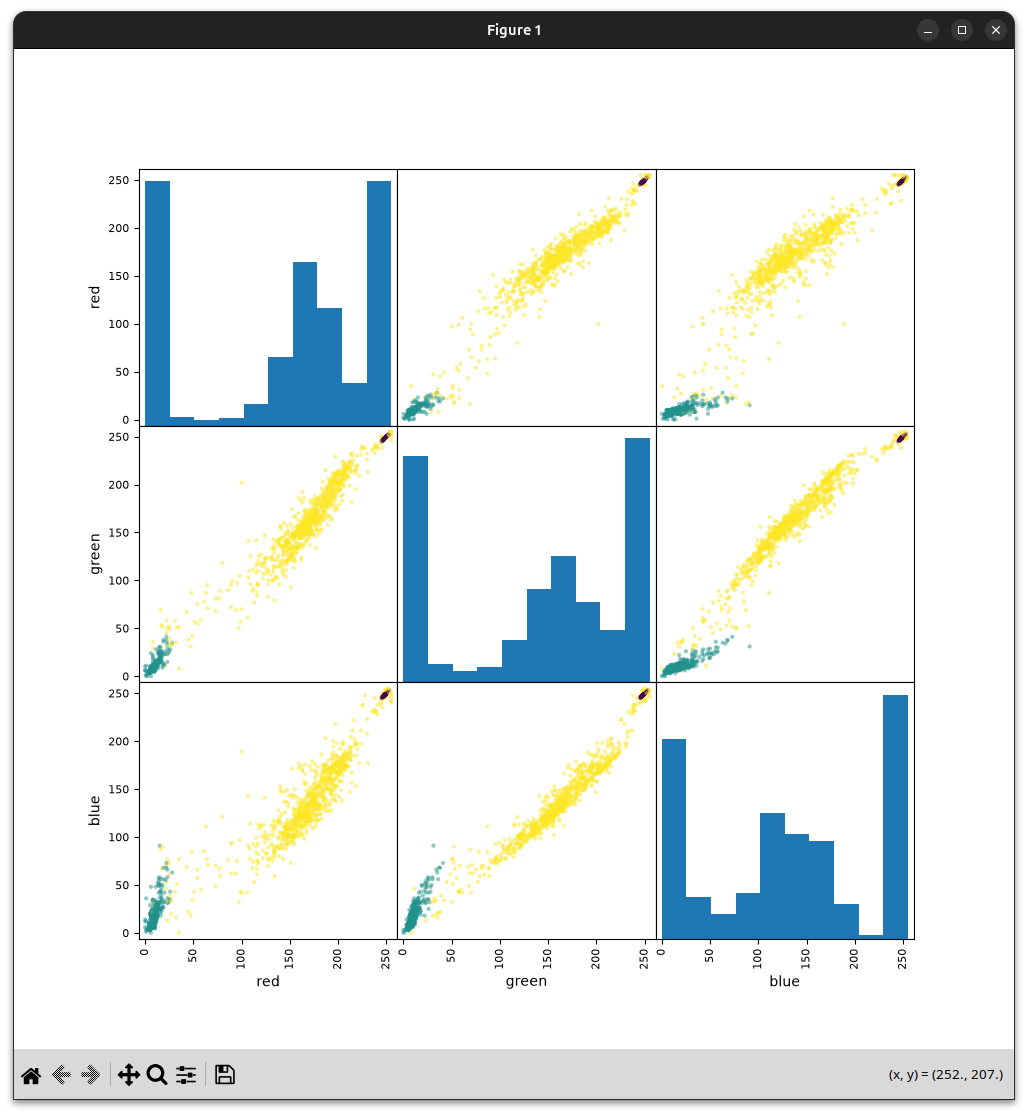
\includegraphics[width=0.75\linewidth]{figure/image23.png}
    \label{fig:placeholder}
\end{figure}

\begin{figure}[H]
    \centering
    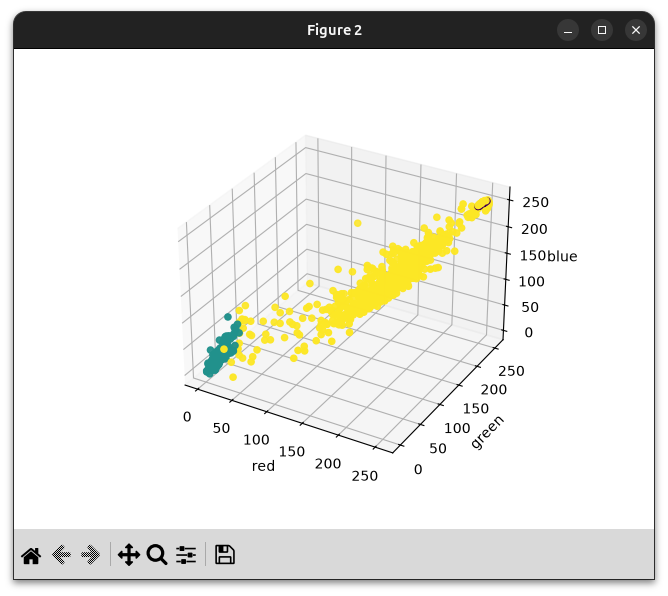
\includegraphics[width=0.75\linewidth]{figure/image24.png}
    \label{fig:placeholder}
\end{figure}

\begin{figure}[H]
    \centering
    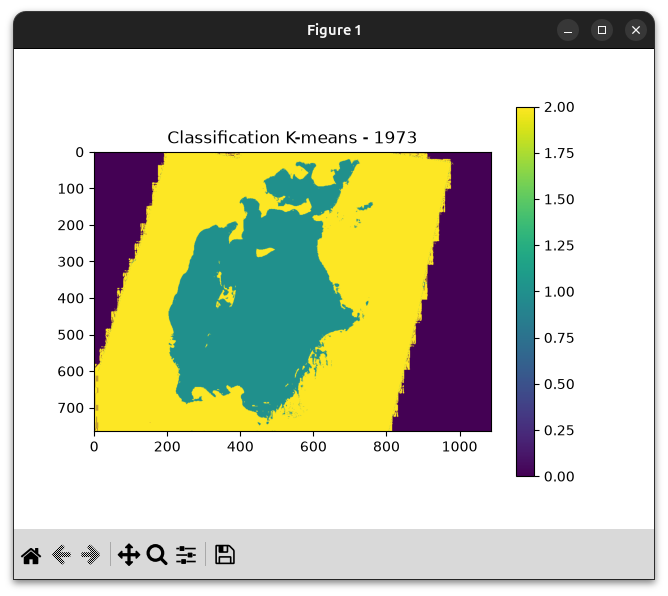
\includegraphics[width=0.75\linewidth]{figure/image25.png}
    \label{fig:placeholder}
\end{figure}

\begin{figure}[H]
    \centering
    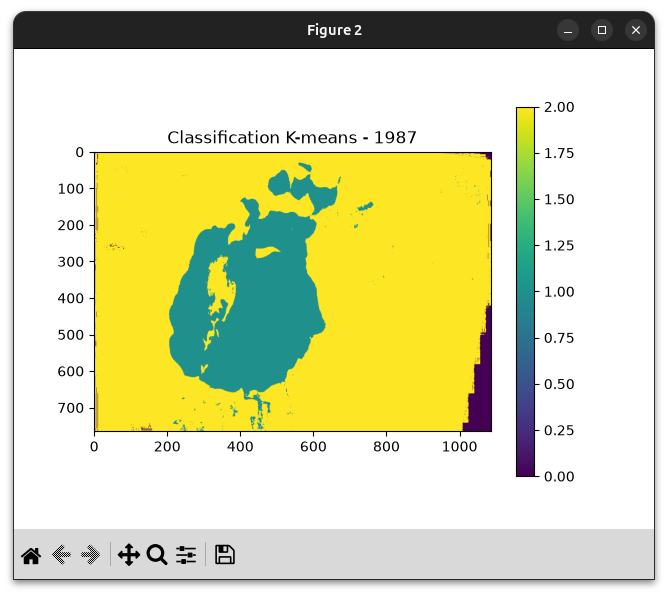
\includegraphics[width=0.75\linewidth]{figure/image26.png}
    \label{fig:placeholder}
\end{figure}

\begin{figure}[H]
    \centering
    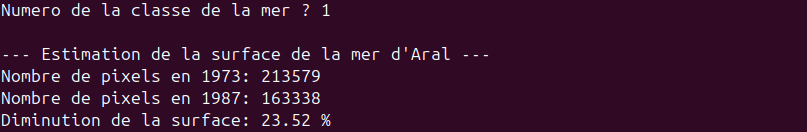
\includegraphics[width=0.75\linewidth]{figure/image27.png}
    \label{fig:placeholder}
\end{figure}


\subsection{| 7.3 Question}

k = 3, full.
\begin{figure}[H]
    \centering
    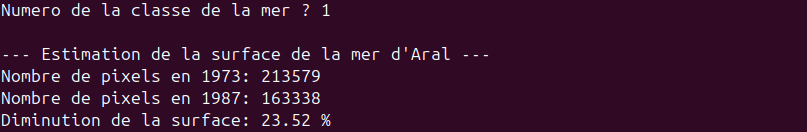
\includegraphics[width=0.75\linewidth]{figure/image27.png}
    \label{fig:placeholder}
\end{figure}

k = 4, full
\begin{figure}[H]
    \centering
    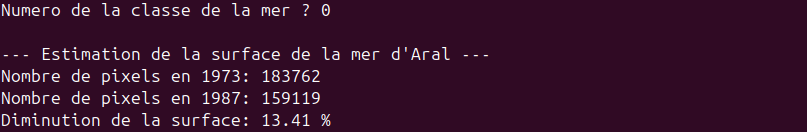
\includegraphics[width=0.75\linewidth]{figure/image28.png}
    \label{fig:placeholder}
\end{figure}

k = 5, full.
\begin{figure}[H]
    \centering
    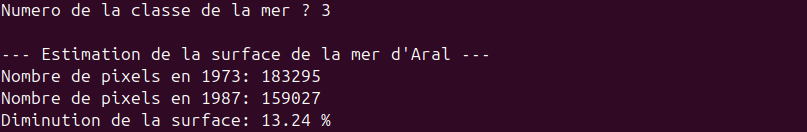
\includegraphics[width=0.75\linewidth]{figure/image29.png}
    \label{fig:placeholder}
\end{figure}

k = 3, diag.
\begin{figure}[H]
    \centering
    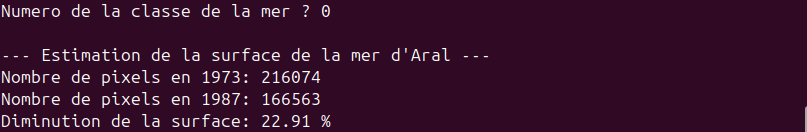
\includegraphics[width=0.75\linewidth]{figure/image30.png}
    \label{fig:placeholder}
\end{figure}

k = 3, spherical.
\begin{figure}[H]
    \centering
    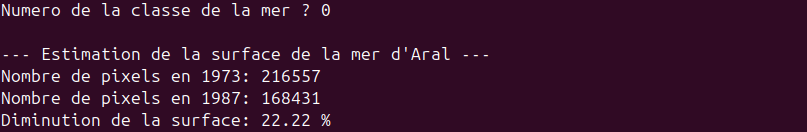
\includegraphics[width=0.75\linewidth]{figure/image31.png}
    \label{fig:placeholder}
\end{figure}

R: On a étudié l’influence des paramètres du GMM sur la classification des pixels.

Avec une covariance de type `full`, on obtient une diminution estimée de 23,52 \% pour K = 3, 13,41 \% pour K = 4 et 13,24 \% pour K = 5. On remarque donc que l’augmentation du nombre de composantes modifie fortement la répartition des pixels entre les classes.

Avec K = 3, on a aussi testé d’autres types de covariance. On obtient 22,91 \% avec `diag` et 22,22 \% avec `spherical`. Ces résultats restent proches de celui obtenu avec `full`.

On peut conclure que le GMM est sensible au choix des paramètres, en particulier au nombre de composantes. La configuration K = 3 donne ici les résultats les plus cohérents.

\subsection{| 7.4 Question}

R: Les deux méthodes permettent de classer les pixels des images et d’estimer l’évolution de la surface de la mer d’Aral.

Le K-means donne des résultats stables, avec une diminution estimée comprise entre 22,74 \% et 24,35 \% selon le nombre de classes. La zone de l’eau est aussi bien identifiée sur les images classifiées.

Le GMM donne de bons résultats avec 3 composantes, par exemple 23,52 \% avec une covariance `full`, 22,91 \% avec `diag` et 22,22 \% avec `spherical`. En revanche, les résultats changent beaucoup quand on augmente le nombre de composantes, avec seulement 13,41 \% pour K = 4 et 13,24 \% pour K = 5.

On peut donc conclure que, dans ce TP, le K-means fournit le résultat le plus robuste et le plus simple à interpréter.


